\chapter{Introduction}
\label{chap:introduction}

\section{Partially Observed Epidemic Count Data}
\label{sec:data_background}

Outbreak data often consist of aggregate counts reported by public health surveillance systems. The data, which typically reflect the incidence or prevalence of cases in the population, are used to develop an understanding of the outbreak dynamics, assess the effectiveness of interventions, and quantify uncertainty about how the outbreak is likely to evolve. The task of modeling an outbreak is complicated by the limited extent of epidemiological data, which are recorded at discrete observation times, commonly describe just one aspect of the disease process, e.g., infections, and usually capture only a fraction of cases. Complete subject--level data, which would consist of full transmission chains and exact times at which individuals transition through disease states, are rarely available. Asymptomatic cases and imperfect surveillance result in systematic underreporting, which makes it difficult to disentangle whether the data arose from a severe outbreak observed with low fidelity, or a mild outbreak where most cases were detected. The challenges involved in characterizing the outbreak dynamics are often further exacerbated by changes in the outbreak dynamics or surveillance over time, which can reduce the effective amount of available information. Hence, fitting models in the absence of complete data is a complicated missing data/latent variable problem. 

\section{Compartmental Epidemic Models}
\label{sec:outbreak_models}

Compartmental epidemic models are used to describe the dynamics of an outbreak, to estimate how features of the population or environment affect its severity, and to understand how interventions might help to disrupt transmission. A compartmental model represents the time--evolution of an outbreak in terms of the disease histories of individuals as they transition between discrete states, or model compartments. When we use a compartmental model to describe the \textit{transmission} dynamics of an outbreak, the compartments encode structural information about how individuals at different infection states interact to transmit the infectious agent. In contrast, states in a compartmental model for \textit{disease} dynamics typically correspond to discrete stages in the natural history of within--host disease progression without necessarily referring to a host's transmissive potential. 

A compartmental model is referred to as a mechanistic model when it prescribes physical laws that govern the transmission dynamics of an outbreak. For example, the model might specify the rates of infectious contact between classes of individuals, or with an environmental reservoir that is a vector for transmission. The mechanistic structure of the model specifies a functional form for the temporal, and possibly spatial, spread of the epidemic process that is coarsely reflected in incidence and prevalence data. In contrast with their mechanistic counterparts, phenomenological models describe the incidence process without explicit reference to the physical system that is under observation \cite{chowell2016review,chowell2017fitting}. The price we pay for adopting a mechanistic approach is that our models will be obviously ``wrong", at least in the sense that all models are wrong, so it will be our responsibility to justify their reasonableness. Our reward is that mechanistic models provide us with interpretable, generative descriptions of outbreak dynamics. Moreover, the ubiquity of mechanistic models in the epidemiological literature enables us to incorporate information from previous studies into our own models to inform our prior beliefs about specific aspects of the transmission dynamics. Historical overviews of mechanistic models for disease transmission may be found in \cite{anderson1992infectious,brauer2017mathematical,keeling2008,lessler2016mechanistic}.

Mechanistic compartmental models can be specified at varying levels of fidelity to the underlying epidemic process. Our models will range in granularity, from agent--based models in which we explicitly track the disease histories of individuals, to population--level models defined by the aggregate flow of individuals between model compartments. We refer to a mechanistic model as a stochastic epidemic model (SEM) when we model stochasticity in the epidemic process. Compartmental models with complex dynamics have historically represented the epidemic process as deterministic systems of ordinary differential equations \cite{keeling2008}. All of the models in this dissertation will treat the epidemic process as evolving continuously in time, but observed at discrete times. The decision to work with continuous--time models is advantageous when observation times are not evenly spaced, or when various sub--processes evolve on different time scales \cite{glass2003,shelton2014}. Discrete time models generally produce results that are not independent of the choice time--step, and can be problematic when the census interval of the data and the generation time of the epidemic are misaligned (see \cite{shelton2014} for examples). One (very) compelling reason to prefer discrete time models is that the computational effort required to fit discrete time models can be quite low in settings where it is possible to approximate the transition densities of the epidemic process with common statistical distributions \cite{fisher2017time,held2005}. 

The statistical questions and computational challenges involved in fitting compartmental models are different in small and large population settings. 
It is particularly important to account for stochasticity in the epidemic process when the population size is small since randomness in the disease process at the subject level can substantially affect the propensity of an infectious agent to spread. 
As we shall see, fitting a SEM to partially observed count data requires that we enumerate the possible epidemic paths from which the data could have arisen. This can be a daunting task since the set of possible epidemic paths is potentially huge, and the stochastic processes used to model outbreaks in small populations are not always amenable to approximation. In contrast, outbreaks in large, well--mixed populations are often amenable to a variety of approximations that will enable us to fit models with complex dynamics. However, as we shall see, various aspects of these models will interact in complicated ways that require us to think carefully about computation and parameterization. 

In this dissertation, we contribute computational methods for fitting continuous time SEMs to partially observed epidemic count data in both small and large populations. In spite of the rather obvious ubiquity and importance of this data setting, there is a dearth of computational tools for fitting SEMs that are simple, broadly applicable, and computationally robust. The remainder of this chapter provides an overview of the datasets that motivate our methods, which will also serve to outline the organization of this dissertation. 

\section{Motivating Examples}
\label{sec:motivating_examples}

\subsection{Influenza in a British Boarding School}
\label{subsec:bbs_descrip}

In our first application, we will analyze data from an outbreak of influenza in a British boarding school \citep{anon1978, davies1982}. This outbreak took place shortly after the Easter term began in January 1978, and was estimated to eventually infect roughly 90\% of the 763 boys aged 10--18. Daily counts of the boys who were confined to the infirmary from January $22^{nd}$ through February $4^{th}$ were accessed via the \texttt{pomp} package in \texttt{R} \citep{pomp}.

\begin{figure}[htbp]
	\centering
	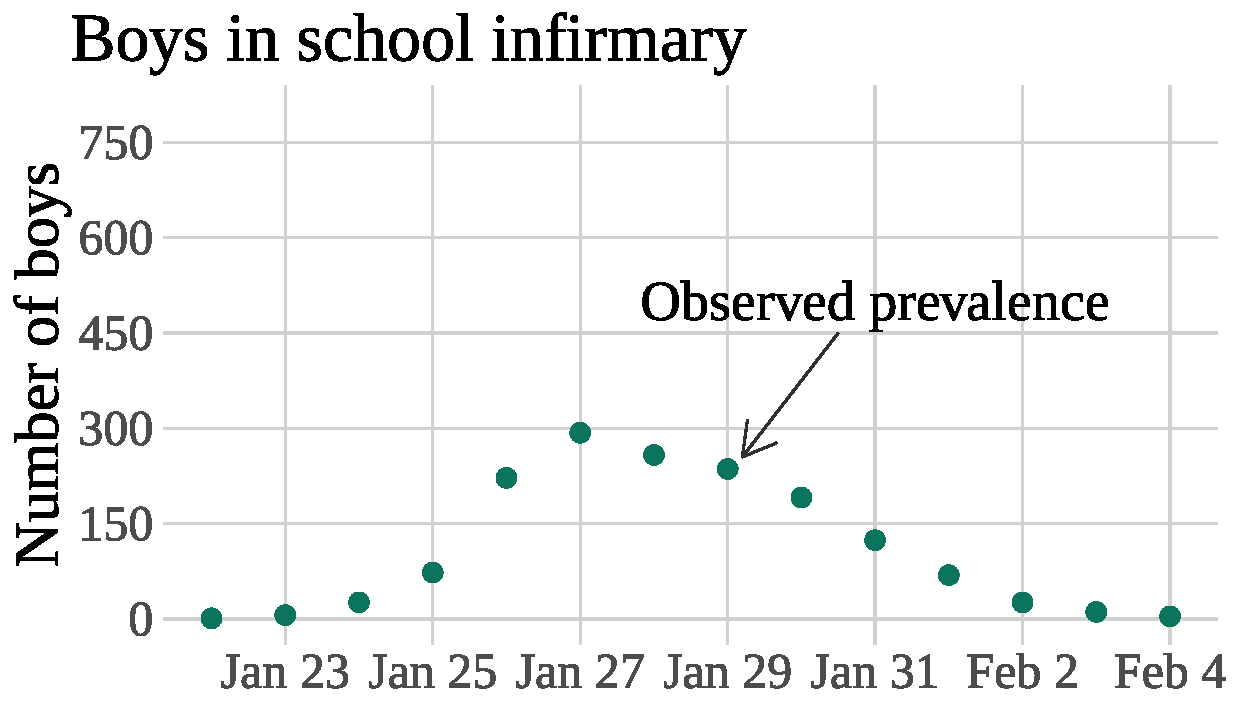
\includegraphics[width=0.6\linewidth]{figures/bbs_data}
	\caption{Data from an outbreak of influenza in a British boarding school.}
	\label{fig:bbsdata}
\end{figure}

Although this dataset is small in scale and duration, reconstructing the true path of the outbreak and describing its dynamics are highly non--trivial inferential tasks. Complicating matters is the lack of individual--level information of any sort, along with the possibility that not all of the boys who were infectious on a given day were successfully detected and isolated. In Chapter  \ref{chap:bda_for_fitting_sems_to_prevalence_data}, we present a computationally efficient algorithm for fitting stochastic epidemic models to partially observed prevalence data in small to moderate size populations. This work has been published in \cite{fintzi2017efficient}. 

\subsection{Epidemics in Large Populations}
\label{subsec:largepop}

\subsubsection{Ebola in West Africa, 2013--2015}
\label{subsec:ebola_descrip}

Starting in December 2013, the West African countries of Guinea, Liberia, and Sierra Leone experienced an outbreak of Ebola that was unprecedented in its size and duration compared to previous Ebola outbreaks. The first cases were thought to have occurred in December 2013 in the Gu\'{e}d\'{e}ckou prefecture in Guinea, while the first cases in Liberia and Sierra Leone were detected on March 30 and June 12, 2014, respectively. By March 2016, a total of 28,646 suspected, probable, and confirmed cases had been reported along with 11,323 deaths \cite{who2016situation}. The outbreak was exacerbated by a number of factors including insufficient outbreak response infrastructure, highly transient populations, and failures to engage with communities early on in the outbreak to implement infection prevention and control measures \cite{coltart2017ebola,dudas2017virus}. 

\begin{figure}[htbp]
	\centering
	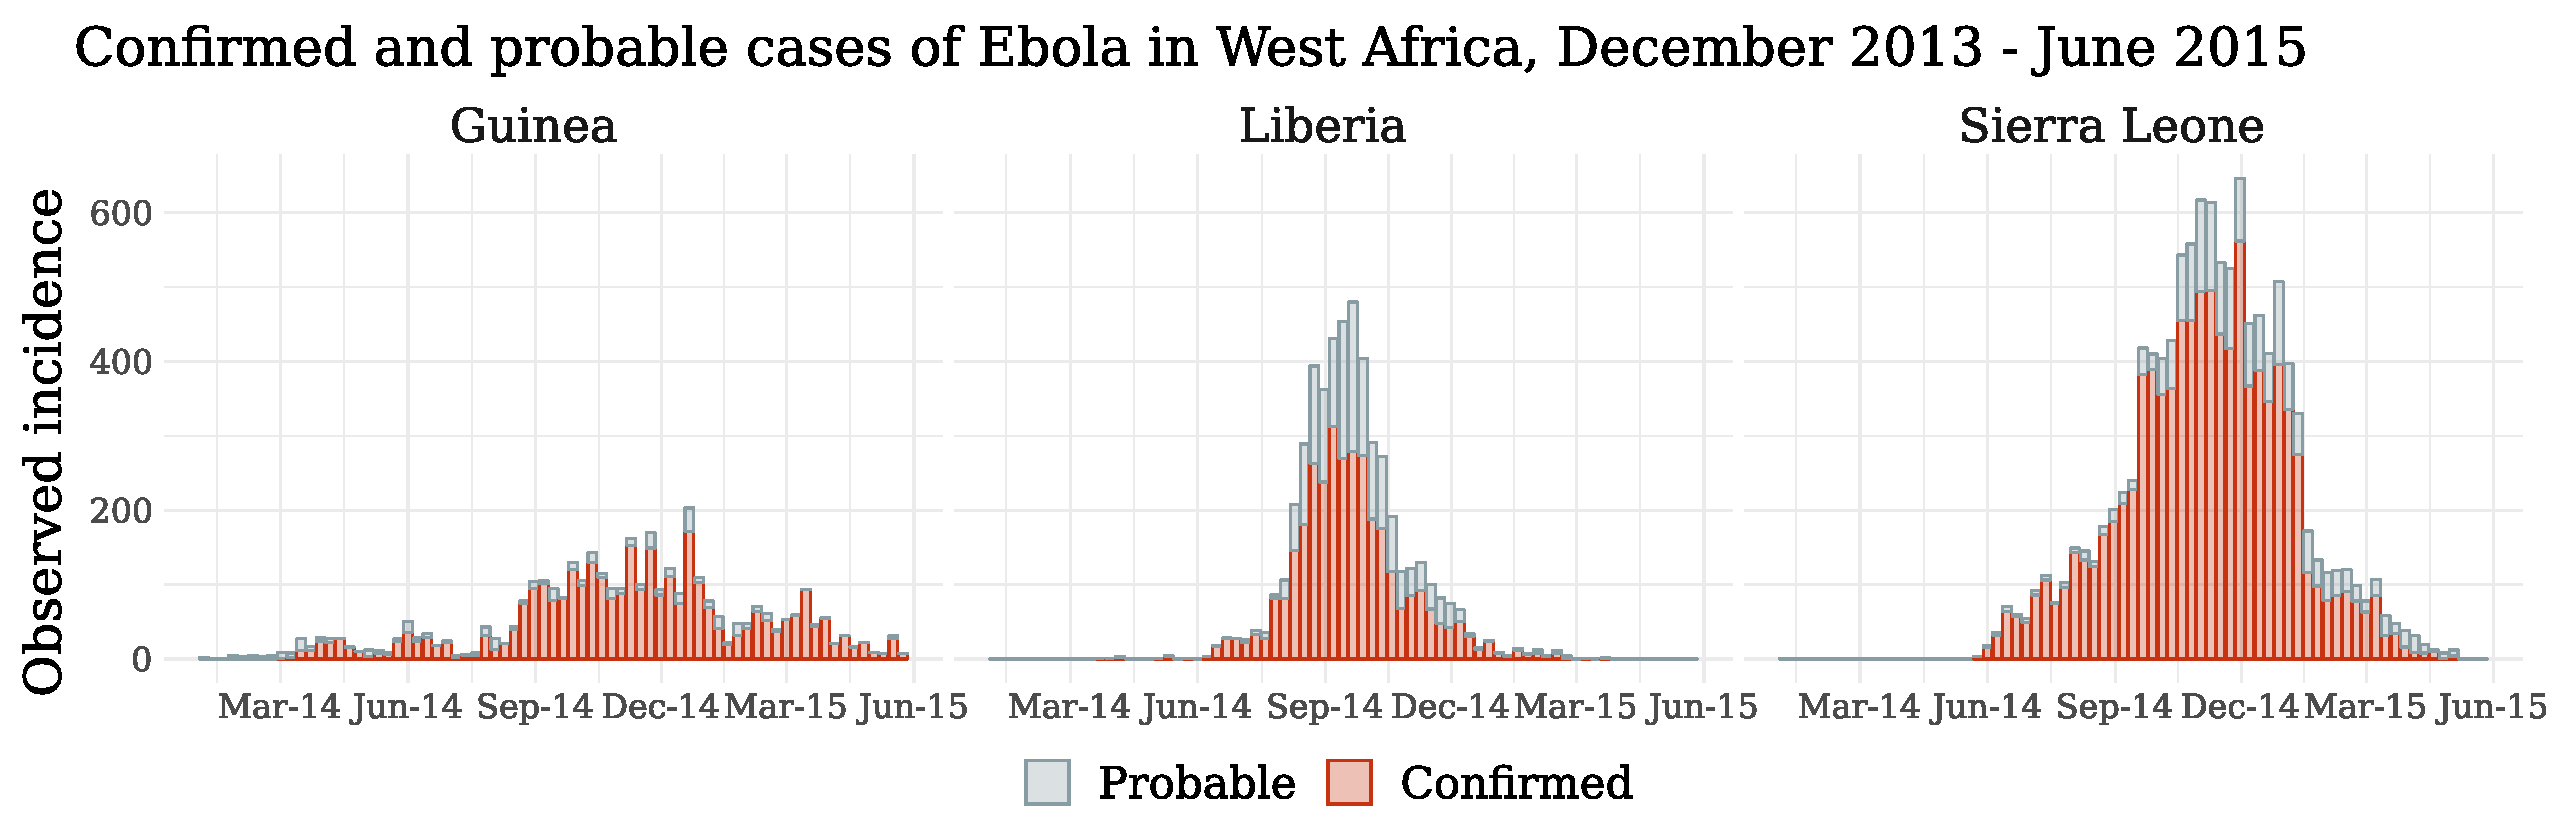
\includegraphics[width=\linewidth]{figures/ebola_dat}
	\caption{Weekly incidence of confirmed and probable cases of Ebola in Guinea, Liberia, and Sierra Leone.}
	\label{fig:eboladat_intro}
\end{figure}

There are several reasons to suspect that the true incidence is significantly under--counted in the dataset. First, suspected cases accounted for sizable fractions of the total case counts, particularly in  Liberia, but were not available as part of this dataset (Table \ref{tab:ebola_descriptives_intro}). Furthermore, analyses based on phylogenetic data \cite{scarpino2014epidemiological} and case fatality ratios \cite{atkins2015under,garske2017heterogeneities} suggest that many cases may have gone undetected, particularly in the early stages, and during the peak, of the outbreak when health systems were overwhelmed. 

\begin{table}[htbp]
	\caption[Ebola incidence by country and case type]{WHO cumulative Ebola incidence by country and case type through May 24, 2015 \cite{who2016eboladat}. Suspected cases were computed as the difference between the official CDC total \cite{cdc2016eboladat}, which included all three case types, and the WHO confirmed plus probable cases.}
	\label{tab:ebola_descriptives_intro}
	\small
	\centering
	\begin{tabular}{lcccc}	
		\hline	
		& \textbf{Guinea} & \textbf{Liberia} & \textbf{Sierra Leone} & \textbf{Total} \\\hline
		\textbf{Confirmed}$ ^1 $ & 3,210 & 3,342 & 9,494 & 16,044\\ 
		\textbf{Probable}$ ^1 $ & 419 & 1,652 & 1,823 & 3,894 \\
		\textbf{Suspected$ ^2 $} & 12 & 5,672 & 1,389 & 7,073 \\
		\hline
		\textbf{Total} & 3,641 & 10,666 & 12,706 & 27,013 \\
		\hline
		\multicolumn{5}{l}{\scriptsize $ ^1 $ Dataset used in the current analysis, cases through 05--24--2015.}\\
		\multicolumn{5}{l}{\scriptsize $ ^2 $ Not available as part of the dataset for this analysis.}\\
	\end{tabular} 
\end{table}

Mathematical models were critical to informing decisions about resource allocation and interventions throughout the outbreak \cite{coltart2017ebola}. A review of 66 modeling studies comprising 125 models for the population--level spread of the outbreak found that modelers typically relied on pre--existing publicly available epidemiological data, which most often consisted of aggregate count data such as weekly incidence counts published by the WHO or national ministries of health \cite{chretien2015mathematical}. Modelers working with incidence data were most often interested in describing the transmission dynamics, particularly the basic reproductive number. Other objectives included forecasting the possible time--evolution of the outbreak, and constructing models to assess the effects of various interventions on the transmission dynamics. Although modeling teams working with publicly available data were not always involved in the policy--making process, the importance of developing outbreak models using real--world data, during what for those teams would be "peace time", has been emphasized as a critical exercise in preparing for future outbreaks \cite{viboud2018rapidd}.

Analyzing data from the Ebola outbreak presents, in some ways, a fundamentally different challenge compared to the boarding school data. As will become clear, the population sizes of the three countries are far too large for the small population methods in Chapter \ref{chap:bda_for_fitting_sems_to_prevalence_data} to be used. In Chapter \ref{chap:lna_for_sems}, we present a framework that builds on a linear noise approximation (LNA) for a broad class of compartmental SEMs \cite{fearnhead2014,komorowski2009,ross2009parameter,wilkinson2011stochastic}, and that uses state of the art Markov chain Monte Carlo (MCMC) tools to fit SEMs to partially observed incidence data in large population settings. 

\subsection{Pandemic A(H1N1) Influenza in Finland}
\label{subsec:flu_description}

The emergence of a pandemic influenza A strain, A(H1N1)pdm09, in the spring of 2009 led to widespread concern that it would results in high mortality and excessive stress on public health systems around the world. The strain, commonly referred to as ``swine flu", was a triple reassortment of human, avian, and swine viruses, and was of particular concern because of its similarity to the 1918 pandemic strain that infected up to a third of the world's population and led to an estimated 50 million deaths \cite{cdc1918pandemic}. While the burden imposed by the 2009 pandemic was ultimately comparable to that of seasonal influenza \cite{iuliano2018estimates}, it nevertheless resulted in an estimated 110,000--400,000 respiratory deaths and 50,000--180,000 cardivascular deaths \cite{dawood2012estimated}. The age--standardized cumulative incidence was estimated from serological samples in 19 countries to be between 20\%--27\% of the total population in those countries \cite{van2013estimating}. There was substantial variability in attack rates and transmission dynamics by age, and outbreaks were consistently estimated to be more severe among children and adolescents in terms of cumulative incidence than among adults \cite{opatowski2011transmission,steens2011age,van2013estimating,yang2015inference}. 

We will analyze surveillance data, displayed in Figure \ref{fig:finland_fludat_intro}, from the first and second waves of the epidemic in Finland. The dataset, previously analyzed in \cite{shubin2016revealing} and \cite{shubin2014estimating}, consists of weekly counts of laboratory--confirmed A(H1N1) cases, aggregated into sixteen age strata, that were culled from a national surveillance system \cite{lyytikainen2011surveillance}. For computational considerations, we will further aggregate the data into two age groups, individuals ages 0--19 and those of ages 20+, chosen on basis of differences in mixing patterns, susceptibility, vaccination priority, and observed attack rates \cite{kelly2011age,opatowski2011transmission,steens2011age}. All cases in our dataset were of mild severity, i.e., cases that did not require hospitalization. Following \cite{shubin2016revealing,shubin2014estimating}, we treat all A(H1N1) cases as A(H1N1)pdm09 as nearly all A(H1N1) cases were of the pandemic strain. It is critical to note that the data are not marked by vaccination status.

An important aspect of the pandemic response in Finland was the execution of a concerted vaccination campaign with the adjuvented monovalent vaccine Pandemrix. Each resident was offered one vaccine dose, free of charge, starting in October, 2009. Vaccination priority was given to health care workers, vulnerable individuals, and young people under the age of 20 \cite{syrjanen2014effectiveness}. Coverage levels and the timing of vaccination administration varied by age, see Figure \ref{fig:finland_fludat_intro}, with highest coverage among children under the age of 15 ($ \approx $70\%) and the lowest among young adults between the ages of 20--29 ($ \approx $30\%). In other settings, vaccine efficacy was also found to be higher in children than adults \cite{lansbury2017effectiveness}. Data was not available on vaccine coverage for a trivalent vaccine administered during the 2010--2011 season. 

\begin{sidewaysfigure}[htbp]
	\centering
	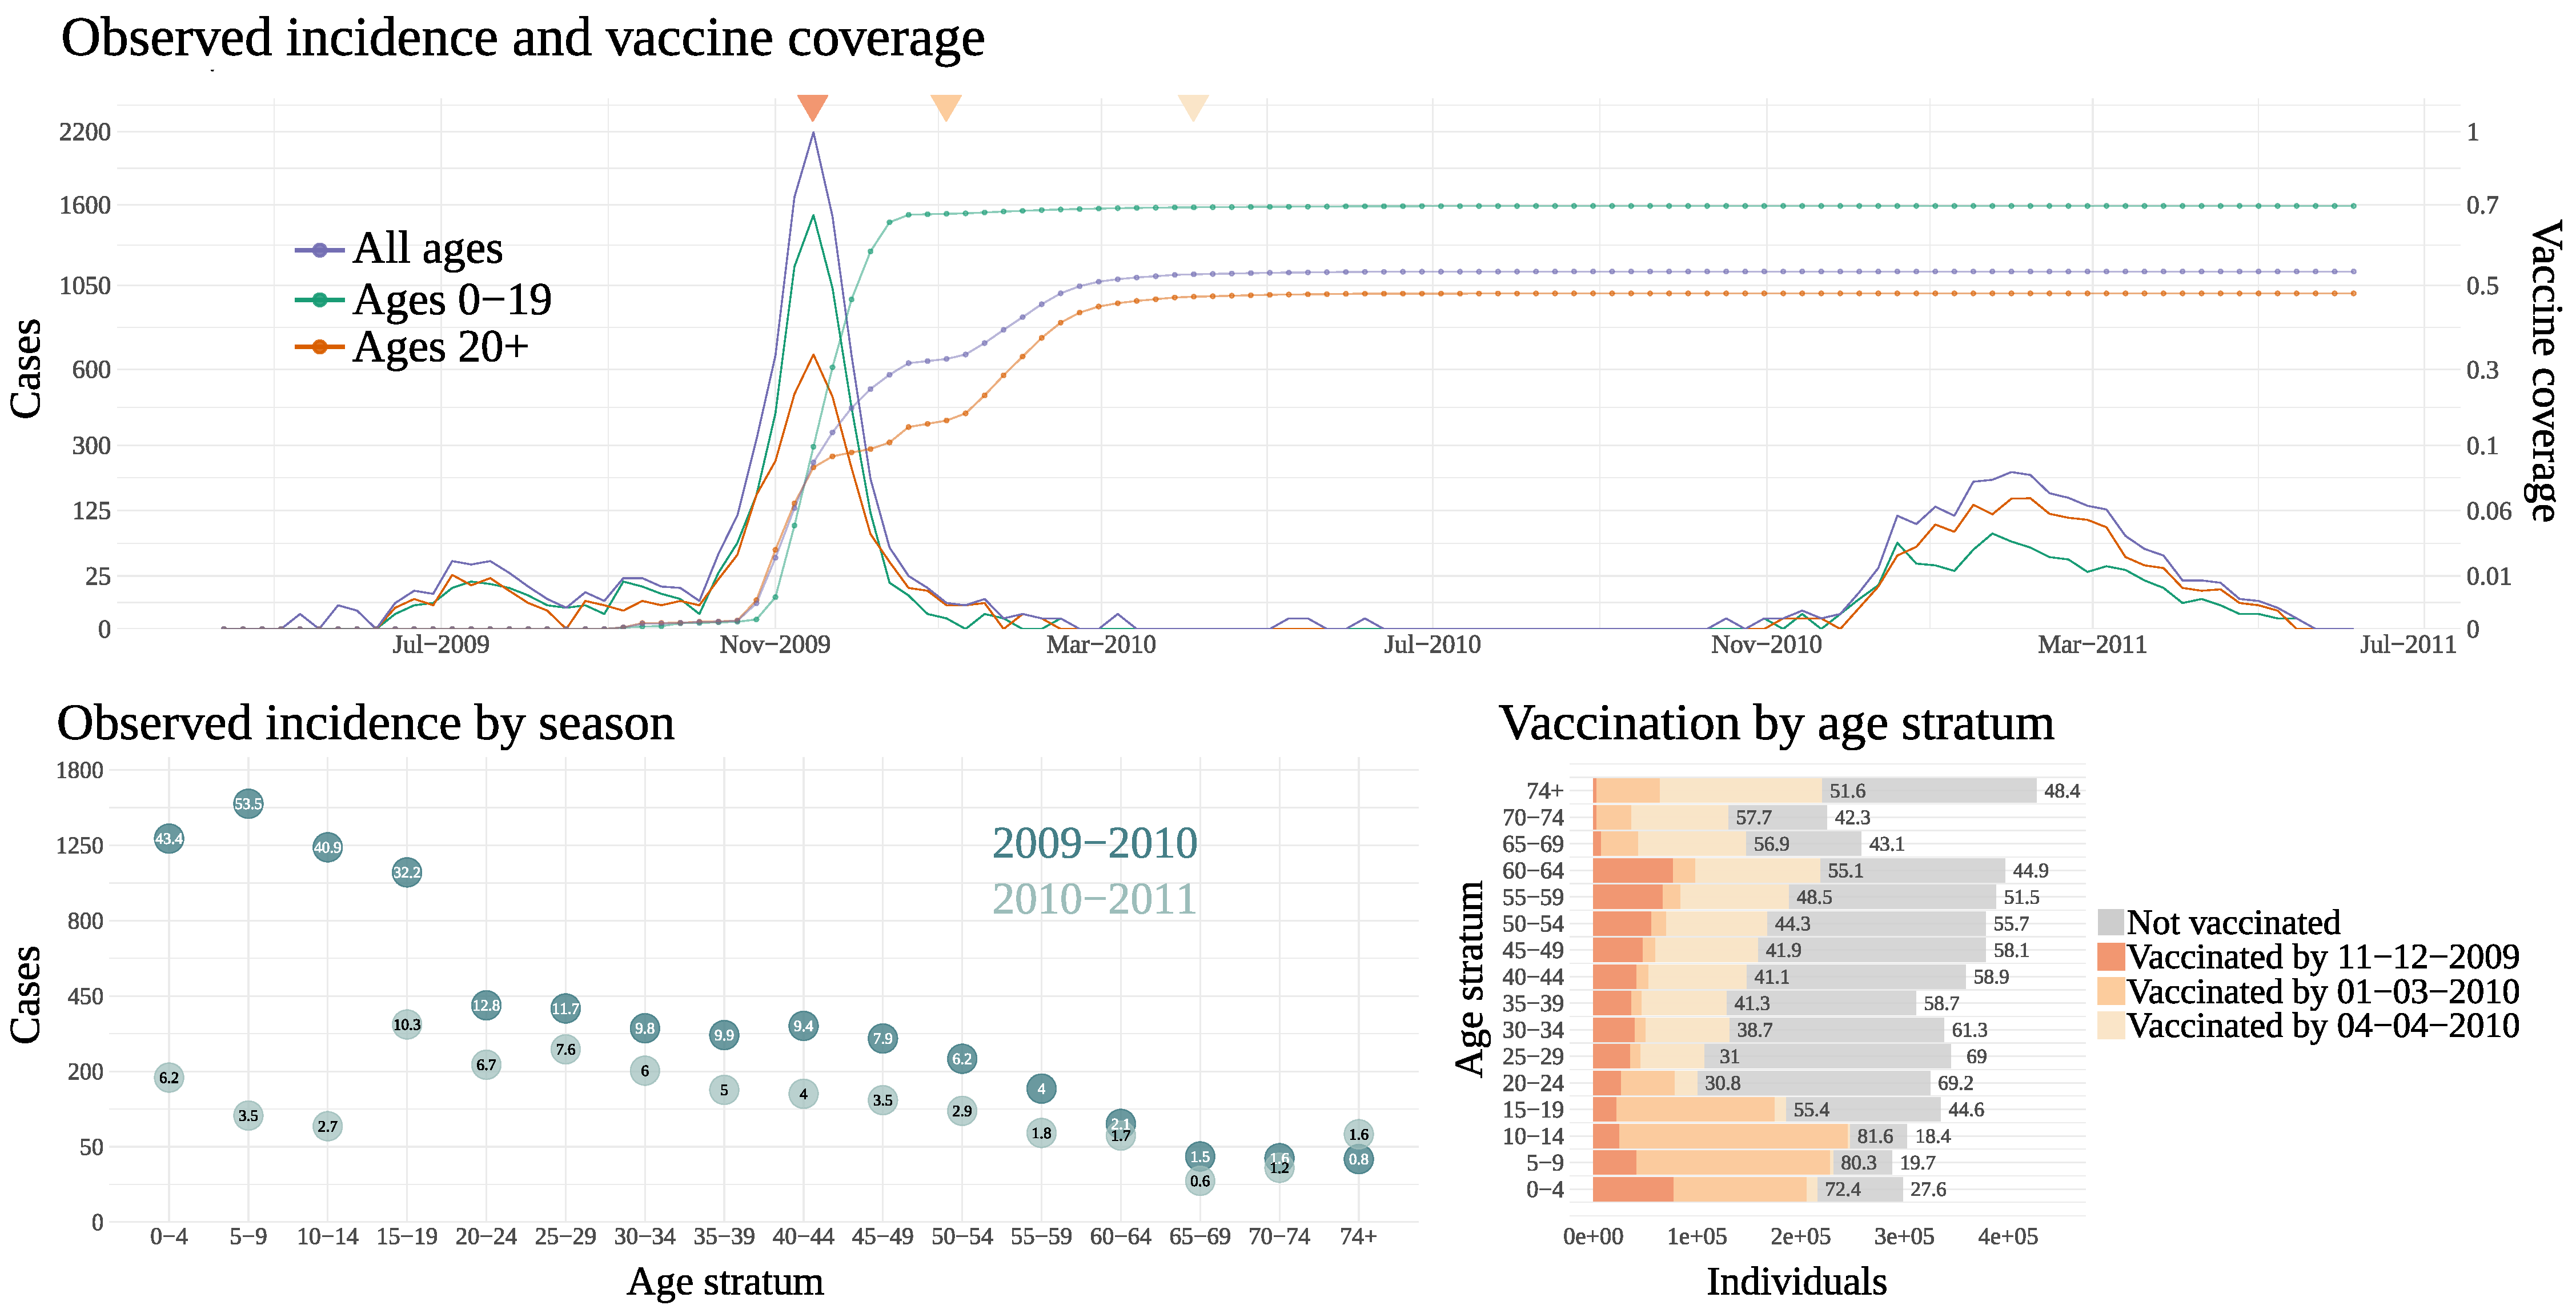
\includegraphics[width=\linewidth]{figures/fludat_plots}
	\caption[A(H1N1)pdm09 incidence and vaccination data from Finland, April 15, 2009 --- June 5, 2011.]{\textbf{Influenza data summaries}. \textit{Top}: Observed incidence (solid lines) and vaccine coverage (lines with points). \textit{Bottom left}: Observed cases by season and age stratum. The 2009--2010 season (dark green) corresponds to the period from April 15, 2009 through April 4, 2010. The 2010--2011 season (light green) corresponds to the period from September 12, 2010 through June 5, 2011. Numbers in points give the attack rate within each stratum for the corresponding season. \textit{Bottom right}: Vaccination coverage by age stratum, colored by vaccine coverages at the times of peak incidence in the first season, tail of the major outbreak in the first season, and end of the vaccination campaign. The numbers inside and outside the histograms denote the percentage of individuals in each stratum that were vaccinated and unvaccinated, respectively, by the end of the vaccination campaign. The times at which vaccine coverages are summarized, denoted by colors of histogram bars, are also identified by corresponding triangles above the top figure.}
	\label{fig:finland_fludat_intro}
\end{sidewaysfigure}

In Chapter \ref{chap:lna_extensions}, we will use methods for approximate inference for SEMs developed and explored in Chapter \ref{chap:lna_for_sems} to fit models with time--varying dynamics. We will then develop an age--vaccination stratified model for the spread of pandemic A(H1N1) in Finland that we will use to pursue three lines of inquiry. First, we will quantify the transmission dynamics and effectiveness of disease surveillance during the first and second seasons. The most important aspect of this involves estimating time--varying reproduction numbers that are interpretable as thresholds for sustained transmission. Second, we will estimate age--specific attack rates and unobserved incidence curves, accounting for underreporting, so that we may better understand the true burden of the pandemic. Finally, we will attempt to understand what effect, if any, the vaccination campaign had in mitigating the severity of the outbreak.